% https://chatgpt.com/share/68eee286-57ec-8005-9314-13a82acff6b5
\raggedbottom
\subsection{Pengujian Sistem Elektronik}
\subsubsection{Hasil Pengujian \emph{Buck Converter} 12V pada \emph{Power Board}}
Pengujian buck converter 12V pada Power Board dilakukan untuk mengevaluasi
kinerjanya pada berbagai kondisi beban. Buck converter dihubungkan dengan
electronic load, sementara arus input dan output diukur menggunakan multimeter,
dan ripple tegangan output dicatat menggunakan osiloskop. Tegangan input
divariasikan pada 16,8V dan 20V, sedangkan arus beban diuji dari 0,5A hingga 5A
dengan langkah 0,5A.

\begin{figure} [H] \centering
  % Nama dari file gambar yang diinputkan
  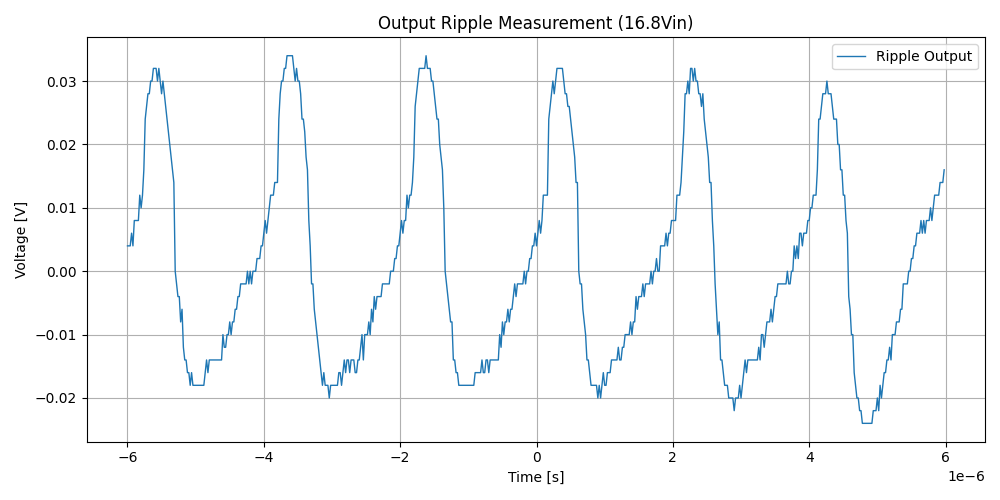
\includegraphics[scale=0.49]{gambar/buck_ripple_16V.png}
  % Keterangan gambar yang diinputkan
  \caption{Ripple Tegangan Output Buck Converter 12V pada VIN 16,8V dan Iout 0.5A}
  % Label referensi dari gambar yang diinputkan
  \label{fig:ripple_16.8V}
\end{figure}
\begin{figure} [H] \centering
  % Nama dari file gambar yang diinputkan
  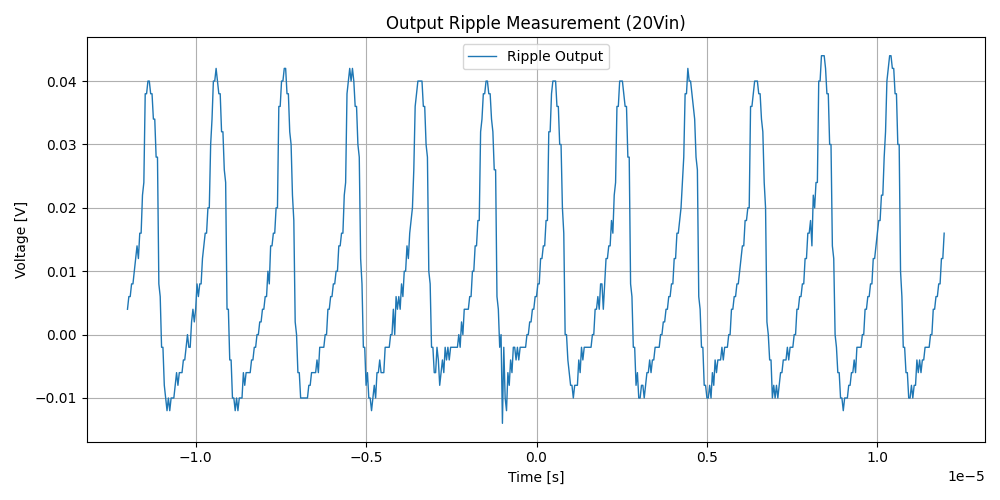
\includegraphics[scale=0.49]{gambar/buck_ripple_20V.png}
  % Keterangan gambar yang diinputkan
  \caption{Ripple Tegangan Output Buck Converter 12V pada VIN 20V dan Iout 0.5A}
  % Label referensi dari gambar yang diinputkan
  \label{fig:ripple_20V}
\end{figure}

\begin{table}[h!]
\centering
\caption{Hasil Pengujian Buck Converter 12V pada VIN 16,8 V}
\label{tab:buck12v_16v_no_vin}
\begin{tabular}{ccccccccc}
\hline
\makecell{VIN\\CONNECTOR} & \makecell{I\_IN\\(A)} & \makecell{I\_OUT\\(A)} & \makecell{V\_OUT\\(V)} & \makecell{P\_IN\\(W)} & \makecell{P\_OUT\\(W)} & EFF & \makecell{V\_OUT\\RIPPLE\\(V)} \\
\hline
16.78 & 0.47 & 0.495 & 12.55 & 7.887 & 6.212 & 0.788 & 0.058 \\
16.75 & 0.91 & 1.058 & 12.55 & 15.243 & 13.278 & 0.871 & 0.062 \\
16.75 & 1.284 & 1.505 & 12.54 & 21.507 & 18.873 & 0.878 & 0.062 \\
16.74 & 1.695 & 1.989 & 12.54 & 28.374 & 24.942 & 0.879 & 0.064 \\
16.74 & 2.118 & 2.48 & 12.54 & 35.455 & 31.099 & 0.877 & 0.068 \\
16.73 & 2.605 & 3.013 & 12.54 & 43.582 & 37.783 & 0.867 & 0.068 \\
16.74 & 3.02 & 3.505 & 12.53 & 50.555 & 43.918 & 0.869 & 0.070 \\
16.72 & 3.501 & 3.958 & 12.53 & 58.537 & 49.594 & 0.847 & 0.074 \\
16.72 & 3.94 & 4.45 & 12.52 & 65.877 & 55.714 & 0.846 & 0.078 \\
16.71 & 4.428 & 5.03 & 12.52 & 73.992 & 62.976 & 0.851 & 0.078 \\
\hline
\end{tabular}
\end{table}
\begin{table}[h!]
\centering
\caption{Hasil Pengujian Buck Converter 12V pada VIN 20 V}
\label{tab:buck12v_20v_no_vin}
\begin{tabular}{ccccccccc}
\hline
\makecell{VIN\\CONNECTOR} & \makecell{I\_IN\\(A)} & \makecell{I\_OUT\\(A)} & \makecell{V\_OUT\\(V)} & \makecell{P\_IN\\(W)} & \makecell{P\_OUT\\(W)} & EFF & \makecell{V\_OUT\\RIPPLE\\(V)} \\
\hline
19.92 & 0.427 & 0.496 & 12.55 & 8.506 & 6.225 & 0.732 & 0.082 \\
19.91 & 0.79 & 0.995 & 12.55 & 15.729 & 12.487 & 0.794 & 0.084 \\
19.90 & 1.099 & 1.45 & 12.54 & 21.870 & 18.183 & 0.831 & 0.088 \\
19.89 & 1.47 & 1.972 & 12.54 & 29.238 & 24.729 & 0.846 & 0.088 \\
19.87 & 1.822 & 2.462 & 12.53 & 36.203 & 30.849 & 0.852 & 0.092 \\
19.86 & 2.2 & 2.966 & 12.53 & 43.692 & 37.164 & 0.851 & 0.092 \\
19.84 & 2.567 & 3.454 & 12.52 & 50.929 & 43.244 & 0.849 & 0.094 \\
19.88 & 2.94 & 3.947 & 12.52 & 58.447 & 49.416 & 0.845 & 0.098 \\
19.78 & 3.334 & 4.45 & 12.48 & 65.947 & 55.536 & 0.842 & 0.102 \\
19.79 & 3.77 & 5 & 12.48 & 74.608 & 62.400 & 0.836 & 0.106 \\
\hline
\end{tabular}
\end{table}

Ripple tegangan output cenderung meningkat seiring dengan bertambahnya arus
beban. Pada VIN 16,8 V, ripple berkisar 0,058--0,078 V, sedangkan pada VIN 20 V,
ripple meningkat menjadi 0,082--0,106 V\@. Peningkatan ripple ini dapat
dijelaskan oleh pengaruh arus beban yang lebih besar terhadap karakteristik LC
filter pada buck converter, sehingga terjadi fluktuasi tegangan output yang
lebih tinggi. Selain itu, perbedaan efisiensi antara VIN 16,8 V dan 20 V
menunjukkan bahwa converter bekerja lebih optimal pada input yang lebih dekat
dengan tegangan nominal targetnya, karena rugi-rugi switching relatif lebih
kecil.

Secara keseluruhan, pengujian ini menunjukkan bahwa buck converter 12V pada
Power Board memiliki performa yang stabil dan efisien untuk rentang beban 0,5--5
A, dengan tegangan output yang konsisten dan ripple yang masih berada dalam
batas aman untuk sistem elektronik yang sensitif. Data ini menjadi dasar untuk
mengevaluasi kesesuaian converter dalam sistem dan mendukung desain rangkaian
daya selanjutnya

\subsubsection{Hasil Pengujian \emph{Buck Converter} 5V pada \emph{Power Board}}
\begin{figure} [H] \centering
  % Nama dari file gambar yang diinputkan
  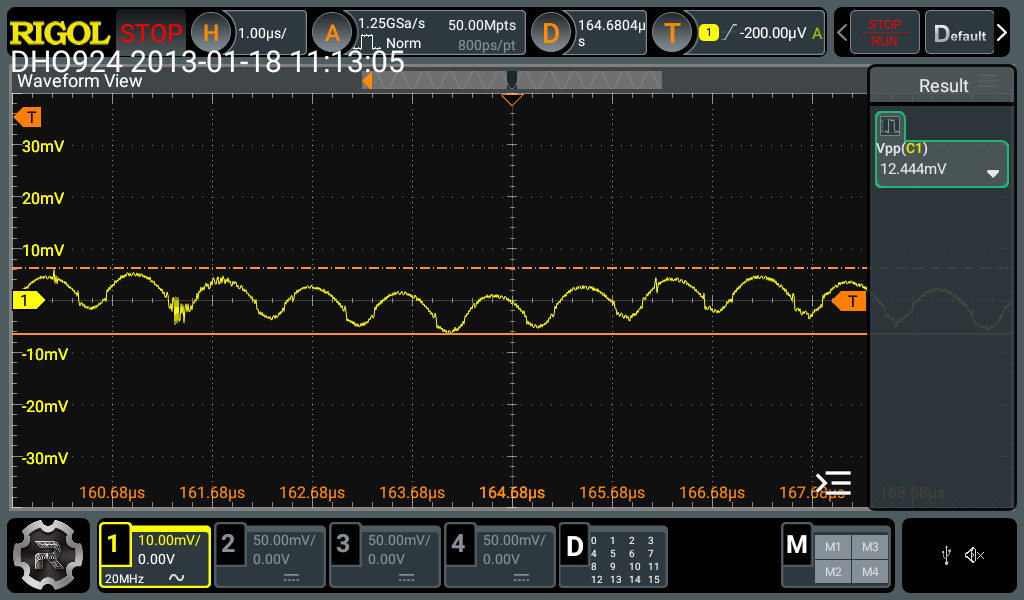
\includegraphics[scale=0.4]{gambar/shita_5v_16Vin.png}
  % Keterangan gambar yang diinputkan
  \caption{Ripple Tegangan Output Buck Converter 5V pada VIN 16,8V dan Iout 0.1A}
  % Label referensi dari gambar yang diinputkan
  \label{fig:5V_shita_16V}
\end{figure}
\begin{figure} [H] \centering
  % Nama dari file gambar yang diinputkan
  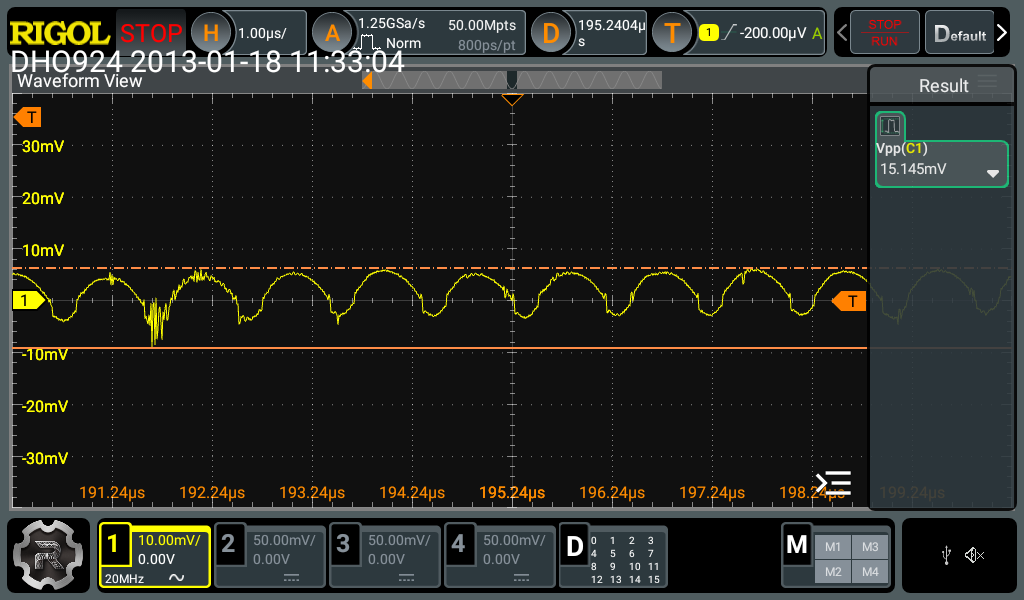
\includegraphics[scale=0.4]{gambar/shita_5v_20Vin.png}
  % Keterangan gambar yang diinputkan
  \caption{Ripple Tegangan Output Buck Converter 5V pada VIN 20V dan Iout 0.1A}
  % Label referensi dari gambar yang diinputkan
  \label{fig:5V_shita_20V}
\end{figure}

\begin{table}[H]
\centering
\caption{Hasil Pengujian Buck Converter 5V pada VIN 16,8 V}
\label{tab:buck5v_16v8}
\begin{tabular}{ccccccccc}
\hline
\makecell{VIN\\CONNECTOR} & \makecell{I\_IN\\(A)} & \makecell{I\_OUT\\(A)} & \makecell{V\_OUT\\(V)} & \makecell{P\_IN\\(W)} & \makecell{P\_OUT\\(W)} & EFF & \makecell{V\_OUT\\RIPPLE\\(V)} \\
\hline
16.8 & 0.144 & 0.198 & 5.00 & 2.4192 & 0.990 & 0.409 & 0.01244 \\
16.8 & 0.209 & 0.390 & 5.00 & 3.5112 & 1.950 & 0.555 & 0.01350 \\
16.8 & 0.275 & 0.593 & 5.00 & 4.6200 & 2.965 & 0.642 & 0.01320 \\
16.8 & 0.337 & 0.784 & 5.00 & 5.6616 & 3.920 & 0.692 & 0.01370 \\
16.8 & 0.403 & 0.984 & 5.00 & 6.7704 & 4.920 & 0.727 & 0.01412 \\
\hline
\end{tabular}
\end{table}

\begin{table}[H]
\centering
\caption{Hasil Pengujian Buck Converter 5V pada VIN 20 V}
\label{tab:buck5v_20v}
\begin{tabular}{ccccccccc}
\hline
\makecell{VIN\\CONNECTOR} & \makecell{I\_IN\\(A)} & \makecell{I\_OUT\\(A)} & \makecell{V\_OUT\\(V)} & \makecell{P\_IN\\(W)} & \makecell{P\_OUT\\(W)} & EFF & \makecell{V\_OUT\\RIPPLE\\(V)} \\
\hline
20.0 & 0.150 & 0.197 & 5.00 & 3.000 & 0.985 & 0.328 & 0.01514 \\
20.0 & 0.207 & 0.390 & 5.00 & 4.140 & 1.950 & 0.471 & 0.01536 \\
20.0 & 0.262 & 0.592 & 5.00 & 5.240 & 2.960 & 0.565 & 0.01604 \\
20.0 & 0.317 & 0.783 & 5.00 & 6.340 & 3.915 & 0.618 & 0.01654 \\
20.0 & 0.376 & 0.983 & 5.00 & 7.520 & 4.915 & 0.654 & 0.01724 \\
\hline
\end{tabular}
\end{table}
Berdasarkan hasil pengujian yang telah dilakukan, \emph{buck converter} 5V pada
\emph{Power Board} menunjukkan kemampuan regulasi tegangan yang baik terhadap
variasi beban. Tegangan keluaran terjaga stabil di sekitar 5~V pada seluruh
kondisi pembebanan, baik ketika tegangan masukan 16,8~V maupun 20~V. Hal ini
menunjukkan bahwa sistem kontrol tegangan pada \emph{buck converter} bekerja
dengan efektif dalam menjaga kestabilan output meskipun terjadi perubahan beban
maupun variasi input.

\subsubsection{Hasil Pengujian \emph{Buck Converter} 5V dan 3.3V pada \emph{Main Board}}
Pengujian \emph{buck converter} pada \emph{Main Board} dilakukan untuk
mengetahui performa konversi daya pada tiga buah \emph{buck converter},
yang terdiri atas dua keluaran 5~V dan satu keluaran 3.3~V. Pengujian dilakukan
dengan menghubungkan masing-masing \emph{buck converter} ke \emph{electronic
load}, di mana arus beban divariasikan dari 0.5~A hingga 3.5~A dengan kenaikan
bertahap sebesar 0.5~A. Tegangan dan arus keluaran diukur menggunakan multimeter,
sedangkan pengamatan terhadap \emph{ripple voltage} dilakukan menggunakan
osiloskop.
\begin{figure} [H] \centering
  % Nama dari file gambar yang diinputkan
  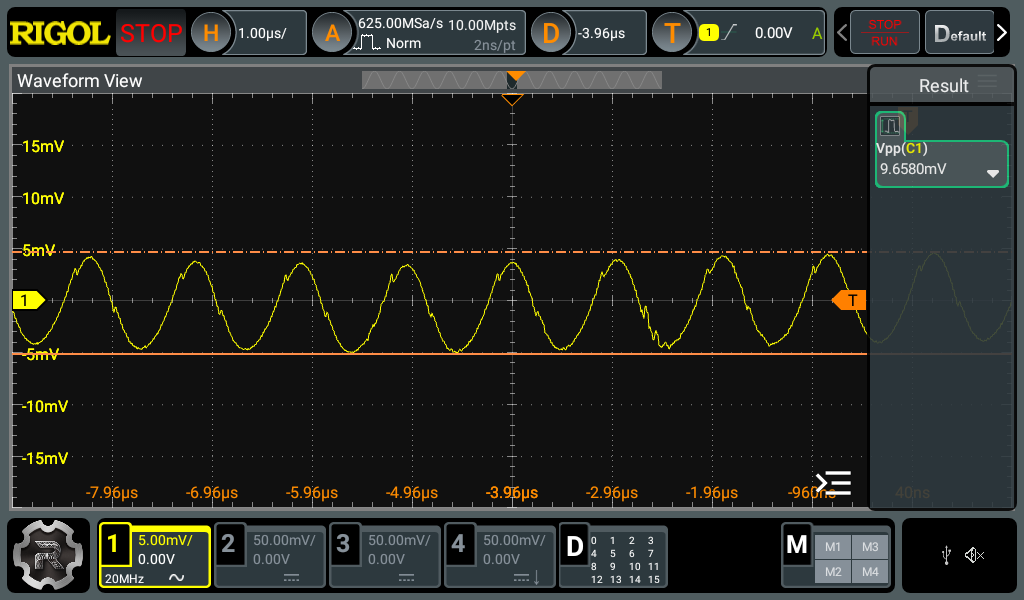
\includegraphics[scale=0.4]{gambar/5V_chikaku.png}
  % Keterangan gambar yang diinputkan
  \caption{Ripple Tegangan Output Buck Converter 5V pada VIN 8.4 dan Iout 0.5A}
  % Label referensi dari gambar yang diinputkan
  \label{fig:5V_chikaku_8V}
\end{figure}
\begin{figure} [H] \centering
  % Nama dari file gambar yang diinputkan
  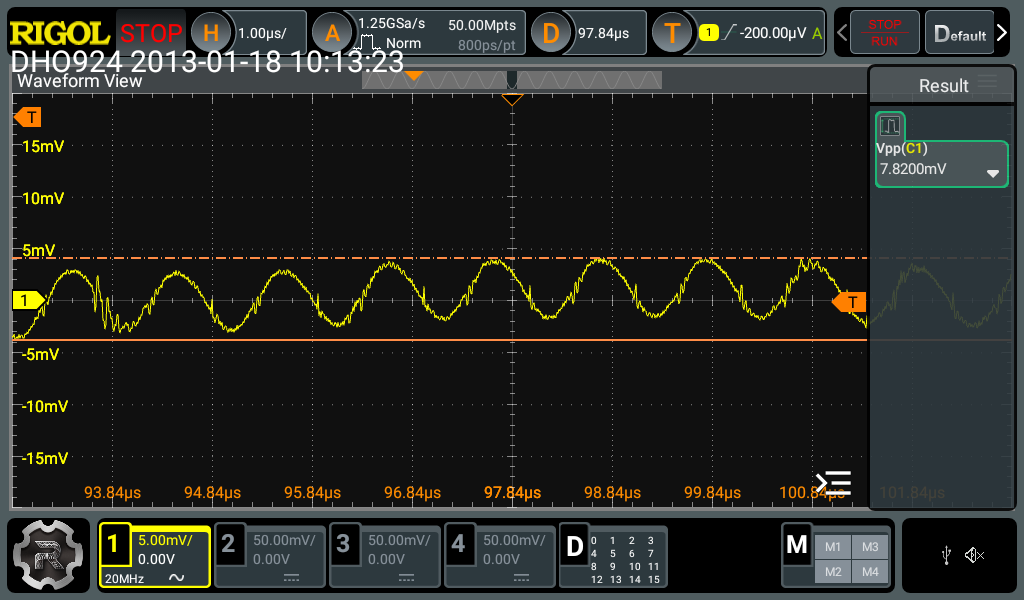
\includegraphics[scale=0.4]{gambar/3v3_chikaku.png}
  % Keterangan gambar yang diinputkan
  \caption{Ripple Tegangan Output Buck Converter 3.3V pada VIN 8.4 dan Iout 0.5A}
  % Label referensi dari gambar yang diinputkan
  \label{fig:3v3_chikaku_8V}
\end{figure}

\begin{table}[H]
\centering
\caption{Hasil Pengujian \emph{Buck Converter} 5V dan 3.3V pada \emph{Main Board}}
\label{tab:buck_mainboard}
\renewcommand{\arraystretch}{1.2}
\setlength{\tabcolsep}{5pt}
\begin{tabular}{cccccccc}
\hline
\makecell{\textbf{V\_IN}\\(V)} & 
\makecell{\textbf{I\_IN}\\(A)} & 
\makecell{\textbf{I\_OUT}\\(A)} & 
\makecell{\textbf{V\_OUT}\\(V)} & 
\makecell{\textbf{P\_IN}\\(W)} & 
\makecell{\textbf{P\_OUT}\\(W)} & 
\makecell{\textbf{Efisiensi}\\(\%)} & 
\makecell{\textbf{V\_OUT}\\\textbf{Ripple (V)}} \\ \hline

\multicolumn{8}{c}{\textbf{Kanal 1 -- Buck Converter 5V}} \\ \hline
8.4 & 0.386 & 0.497 & 5.18 & 3.2424 & 2.57446 & 79.40 & 0.0096 \\
8.4 & 0.714 & 0.991 & 5.18 & 5.9976 & 5.13338 & 85.59 & 0.0100 \\
8.4 & 1.052 & 1.489 & 5.18 & 8.8368 & 7.71302 & 87.28 & 0.0104 \\
8.4 & 1.406 & 1.990 & 5.18 & 11.8104 & 10.3082 & 87.28 & 0.0107 \\
8.4 & 1.783 & 2.485 & 5.18 & 14.9772 & 12.8723 & 85.95 & 0.0106 \\
8.4 & 2.176 & 2.967 & 5.18 & 18.2784 & 15.3691 & 84.08 & 0.0110 \\
8.4 & 2.586 & 3.454 & 5.18 & 21.7224 & 17.8917 & 82.37 & 0.0114 \\ \hline

\multicolumn{8}{c}{\textbf{Kanal 2 -- Buck Converter 5V}} \\ \hline
8.4 & 0.379 & 0.502 & 5.18 & 3.1836 & 2.60036 & 81.68 & 0.00965 \\
8.4 & 0.707 & 0.997 & 5.18 & 5.9388 & 5.16446 & 86.96 & 0.0100 \\
8.4 & 1.041 & 1.493 & 5.18 & 8.7444 & 7.73374 & 88.44 & 0.0103 \\
8.4 & 1.392 & 1.998 & 5.18 & 11.6928 & 10.3496 & 88.51 & 0.0105 \\
8.4 & 1.762 & 2.493 & 5.18 & 14.8008 & 12.9137 & 87.25 & 0.0105 \\
8.4 & 2.153 & 2.987 & 5.18 & 18.0852 & 15.4727 & 85.55 & 0.0108 \\
8.4 & 2.559 & 3.482 & 5.18 & 21.4956 & 18.0368 & 83.91 & 0.0112 \\ \hline

\multicolumn{8}{c}{\textbf{Kanal 3 -- Buck Converter 3.3V}} \\ \hline
8.4 & 0.269 & 0.495 & 3.248 & 2.2596 & 1.60776 & 71.15 & 0.00782 \\
8.4 & 0.473 & 0.987 & 3.248 & 3.9732 & 3.20578 & 80.68 & 0.00786 \\
8.4 & 0.686 & 1.479 & 3.248 & 5.7624 & 4.80379 & 83.36 & 0.00768 \\
8.4 & 0.904 & 1.966 & 3.248 & 7.5936 & 6.38557 & 84.09 & 0.00804 \\
8.4 & 1.130 & 2.456 & 3.248 & 9.4920 & 7.97709 & 84.04 & 0.00815 \\
8.4 & 1.368 & 2.957 & 3.248 & 11.4912 & 9.60434 & 83.58 & 0.00905 \\
8.4 & 1.610 & 3.441 & 3.248 & 13.5240 & 11.17637 & 82.64 & 0.01012 \\ \hline
\end{tabular}
\end{table}
Hasil pengujian ditunjukkan pada Tabel~\ref{tab:buck_mainboard}, yang
memperlihatkan bahwa nilai V\textsubscript{OUT} relatif stabil pada sekitar 5{,
}18~V untuk kedua kanal 5V dan 3{,}248~V untuk kanal 3{,}3V sepanjang rentang
pembebanan. Arus keluaran tercatat berkisar dari 0{,}497~A hingga 3{,}454~A
untuk kanal 5V pertama, 0{,}502~A hingga 3{,}482~A untuk kanal 5V kedua, dan 0{,
}495~A hingga 3{,}441~A untuk kanal 3{,}3V. Efisiensi ketiga \emph{buck
converter} berada pada kisaran 0{,}824--0{,}873 (82{,}4--87{,}3\%) pada beban
menengah dan sedikit menurun pada beban maksimum. Sementara itu, \emph{ripple}
tegangan terukur relatif kecil, berada pada rentang 7{,}8--11{,}4~mV.

\subsubsection{Hasil Pengujian eFuse 5V pada \emph{Power Board}}
Pengujian eFuse 5V pada Power Board dilakukan untuk mengevaluasi kinerjanya
dalam melindungi rangkaian dari kondisi arus lebih. Pada pengujian ini, probe
pertama (warna kuning) dihubungkan ke tegangan pada resistor shunt sebesar
10~m$\Omega$ yang digunakan untuk memantau besarnya arus keluaran, sedangkan
probe kedua (warna biru) dihubungkan ke sisi keluaran \textit{eFuse}. Pada
\emph{power board} ini, nilai trip current yang diatur adalah 0.97A.

\begin{figure} [H] \centering
  % Nama dari file gambar yang diinputkan
  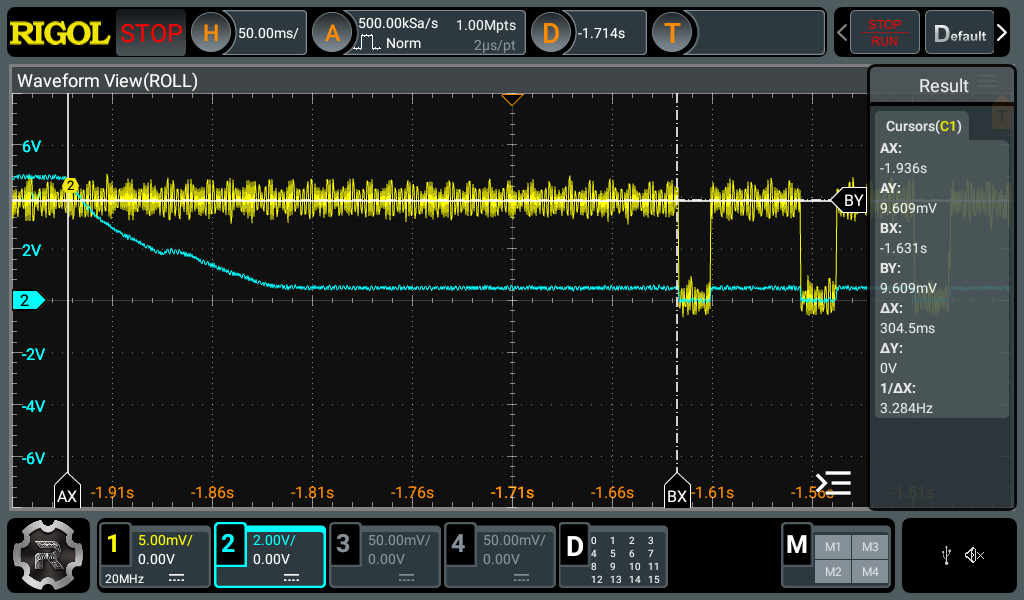
\includegraphics[scale=0.4]{gambar/shita_efuse_trip.png}
  % Keterangan gambar yang diinputkan
  \caption{Respon \emph{trip} efuse 5V pada Power Board}
  % Label referensi dari gambar yang diinputkan
  \label{fig:efuse_5V_shita_trip}
\end{figure}
\begin{figure} [H] \centering
  % Nama dari file gambar yang diinputkan
  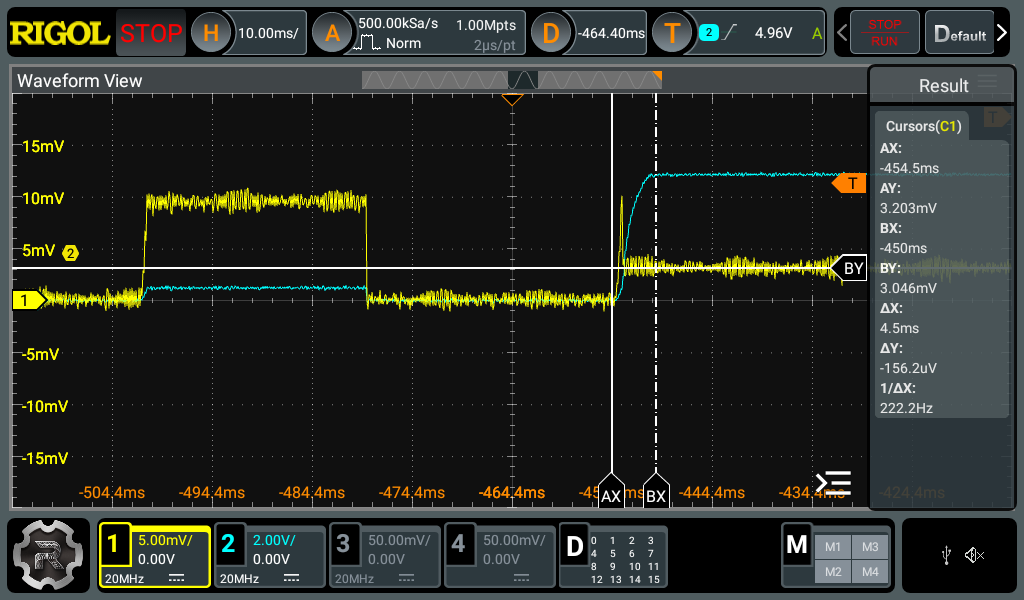
\includegraphics[scale=0.4]{gambar/shita_efuse_recovery.png}
  % Keterangan gambar yang diinputkan
  \caption{Respon \emph{recovery} efuse 5V pada Power Board}
  % Label referensi dari gambar yang diinputkan
  \label{fig:efuse_5V_shita_recovery}
\end{figure}
Pengamatan respon \textit{eFuse} dilakukan menggunakan osiloskop untuk melihat
proses pemutusan (\textit{trip}) dan pemulihan (\textit{recovery}). Berdasarkan
hasil pengamatan yang ditunjukkan pada Gambar~\ref{fig:efuse_5V_shita_trip} dan
\ref{fig:efuse_5V_shita_recovery}, \textit{eFuse} menunjukkan waktu pemutusan
(\textit{trip time}) sekitar 0,3~s, di mana tegangan keluaran menurun dari 4,
52~V menjadi sekitar 0,35~V kemudian arus output dibatasi sebesar 0,97~A hingga
waktu pemutusan selesai. Setelah beban dilepaskan, \textit{eFuse} menunjukkan
waktu pemulihan (\textit{recovery time}) sekitar 0,043~s hingga tegangan
keluaran kembali stabil pada 5V. Hasil ini menunjukkan bahwa \textit{eFuse}
TPS25200 bekerja sesuai dengan karakteristik proteksi arus lebih, yaitu secara
otomatis menghentikan aliran arus ketika beban melebihi batas 1~A, dan
memulihkan keluaran ketika kondisi telah kembali normal.

\subsubsection{Hasil Pengujian eFuse 5V dan 3.3V pada \emph{Main Board}}
Pengujian eFuse pada Main Board dilakukan untuk memastikan fungsi proteksi arus
lebih (\textit{overcurrent protection}) bekerja sesuai dengan batas arus yang
ditentukan. Pengujian dilakukan pada tiga kanal, yaitu eFuse 5 V dengan batas
arus 3.7 A, eFuse 3.3 V dengan batas arus 3,7 A, dan eFuse 3.3 V dengan batas
arus 1 A . Proses pengujian sama seperti sebelumnya, dimana efuse akan dihubungkan
dengan \emph{electronic load} dan shunt resistor 10~m$\Omega$. Tegangan dan arus 
akan diamati melalui osiloskop.

\begin{figure}[H]
    \centering
     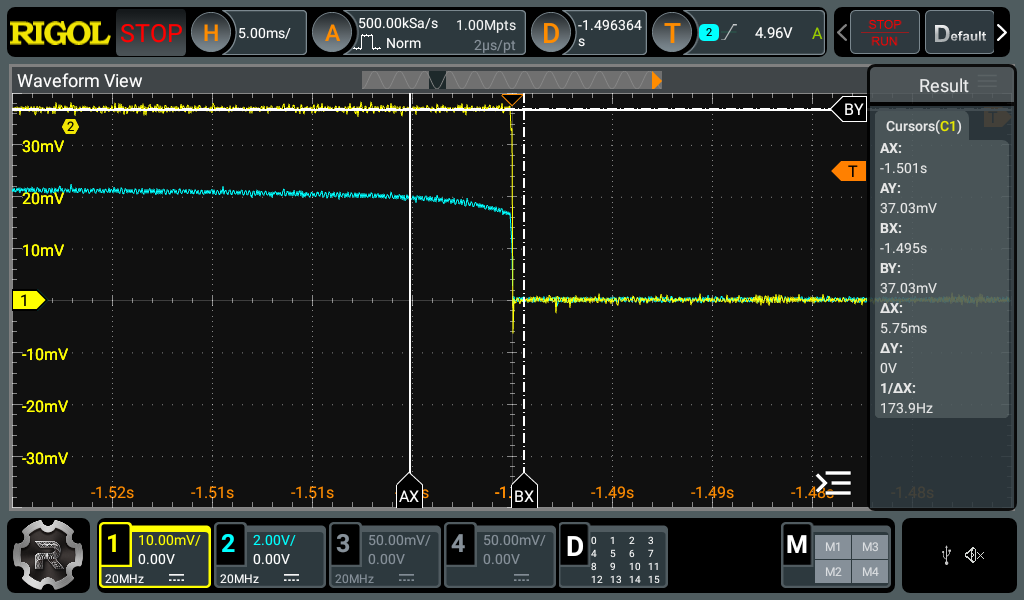
\includegraphics[scale=0.4]{gambar/chikaku_efuse_5v_3.png}
    \caption{Respon \emph{trip} eFuse 5V 3.7A}
    \label{fig:efuse_5v_3A}
\end{figure}
\begin{figure}[H]
    \centering
    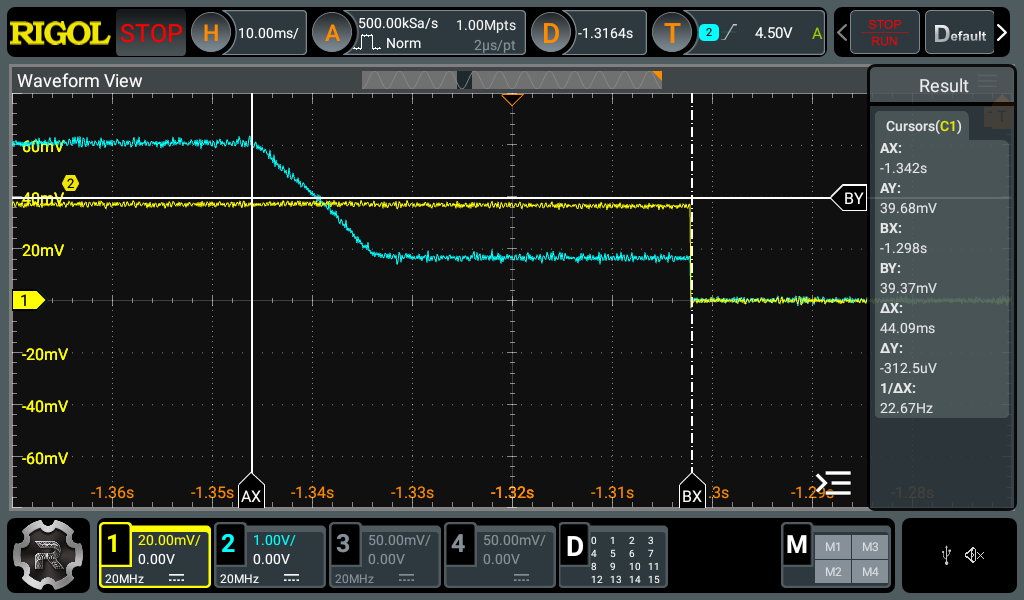
\includegraphics[scale=0.4]{gambar/chikaku_efuse_3v3_3.png}
    \caption{Respon \emph{trip} eFuse 3.3V 3.7A}
    \label{fig:efuse_3v_3A}
\end{figure}
\begin{figure}[H]
    \centering
    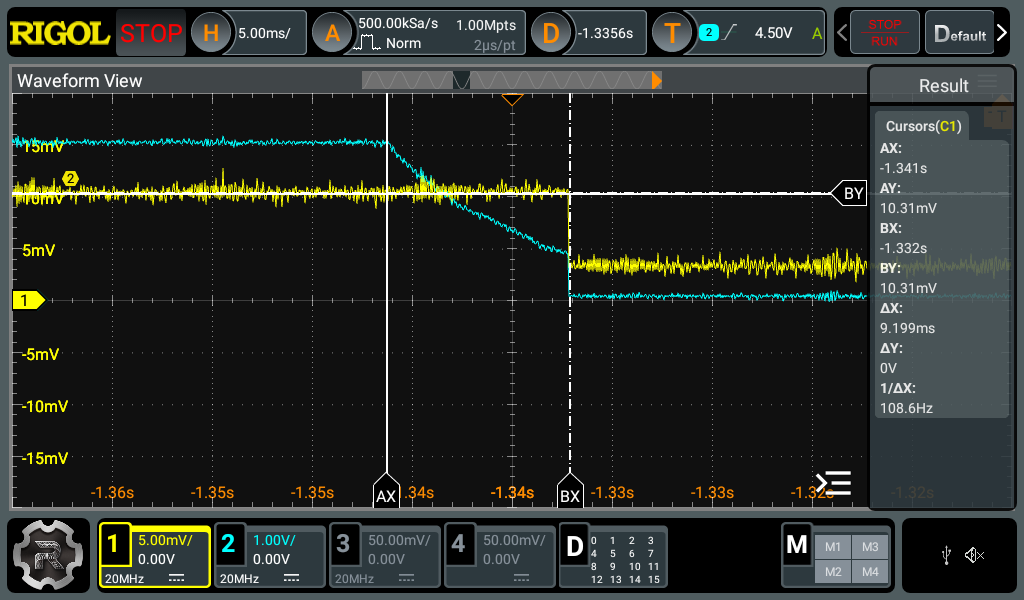
\includegraphics[scale=0.4]{gambar/chikaku_efuse_3v3_1.png}
    \caption{Respon \emph{trip} eFuse 3.3V 1A}
    \label{fig:efuse_3v_1A}
\end{figure}
Berdasarkan hasil pengukuran yang ditunjukkan pada Gambar~\ref{fig:efuse_5v_3A}
hingga Gambar~\ref{fig:efuse_3v_1A}, terlihat bahwa setiap \textit{eFuse}
merespons kondisi arus berlebih dengan melakukan pembatasan arus secara otomatis
hingga mencapai batas \textit{current limit} (ILIM), kemudian memutus keluaran
pada saat batas tersebut terlampaui. Waktu pemutusan bervariasi pada setiap
konfigurasi, dengan estimasi waktu sekitar 5,75~ms pada konfigurasi 5~V 3.7~A,
44,09~ms pada konfigurasi 3,3~V 3,7~A, dan 9,19~ms pada konfigurasi 3.3~V 1~A.

\subsubsection{Hasil Pengujian \emph{Power Selection}}

\subsection{Pengujian Perangkat Lunak}

\subsubsection{Hasil Pengujian Komunikasi STM32 dengan Servo}

\subsubsection{Hasil Pengujian Komunikasi STM32 dengan Jetson Nano}


\subsubsection{Hasil Pengujian Sistem Pembacaan Tegangan Baterai}


\subsection{Pengujian \emph{Motion} Robot}

\subsubsection{Hasil Pengujian Kinematika Gerak Satu Kaki}

\subsubsection{Hasil Pengujian Performa Robot Berjalan Lurus}

\subsubsection{Hasil Pengujian Gerak Lengan Robot}

\subsubsection{Hasil Pengujian Integrasi Gerak Kaki dan Lengan}


\subsection{Pengujian Integrasi Sistem Pada Arena KRSRI 2024}




% \begin{itemize}
%     \item Foto hasil akhir dari PCB Power Board, Main Board, dan Modul STM32 M.2.
%     \item Data uji fungsional mencakup:
%     \begin{itemize}
%         \item Pengujian \textit{buck converter} 5~V dan 12~V. (efisiensi dan kestabilan daya)
%         \item Pembacaan ADC tegangan baterai.
%         \item Respon \textit{electronic fuse (eFuse)} terhadap arus lebih.
%         \item Kestabilan komunikasi servo.
%     \end{itemize}
% \end{itemize}

% \subsection{Hasil Perancangan Firmware STM32}

% \begin{itemize}
%     \item Output komunikasi antara STM32 dan servo (log data, timing paket \textit{Sync Write/Read}).
%     \item Hasil komunikasi antara STM32 dan Jetson Nano melalui USB, mencakup:
%     \begin{itemize}
%         \item Bandwidth komunikasi.
%         \item Latency rata-rata.
%         \item \textit{Packet loss} selama transmisi data.
%     \end{itemize}
%     \item Screenshot atau data dari \textit{serial monitor} yang menunjukkan sistem bekerja dengan benar.
% \end{itemize}
    

% \subsection{Hasil Perancangan Mekanik}

% \begin{itemize}
%     \item Gambar realisasi 3D dan foto prototipe mekanik yang sudah dirakit.
%     \item Data dimensi dan berat aktual dibandingkan dengan rancangan awal.
%     \item Hasil integrasi lengan 6-DOF dan kaki hexapod, seperti:
%     \begin{itemize}
%         \item Jangkauan gerak.
%         \item Radius kerja aktual.
%     \end{itemize}
% \end{itemize}

% \subsection{Hasil Perancangan Perangkat Lunak Robot}

% \begin{itemize}
%     \item Hasil visualisasi gerak kaki/lengan dari simulasi dan real hardware.
%     \item Data uji kinematika berupa perbandingan antara posisi \textit{end-effector} dan target (error posisi).
%     \item Tampilan GUI atau terminal pada Jetson Nano yang menunjukkan hasil visualisasi atau status sistem.
% \end{itemize}

% \subsection{Hasil Integrasi Sistem}

% \begin{itemize}
%     \item Dokumentasi sistem saat bekerja secara penuh (hexapod bergerak dan menggerakkan lengan).
%     \item Data performa sistem, meliputi:
%     \begin{itemize}
%         \item Waktu booting Jetson Nano.
%         \item Total konsumsi daya sistem.
%         \item Sinkronisasi komunikasi Jetson–STM32.
%     \end{itemize}
%     \item Hasil pengujian di arena KRSI:
%     \begin{itemize}
%         \item Kecepatan gerak robot.
%         \item Kemampuan mengambil objek.
%         \item Kestabilan gerakan selama pengujian.
%     \end{itemize}
% \end{itemize}